\documentclass[11pt,a4paper]{article}
\usepackage[utf8]{inputenc}
\usepackage{amsthm, amsmath, mathtools, amssymb}
\usepackage[left=2.8cm,right=2.8cm,top=3cm,bottom=3cm]{geometry}
\usepackage[colorlinks, linkcolor=blue, citecolor=blue, urlcolor=blue]{hyperref}
\usepackage{dsfont}
\usepackage{xcolor}
\usepackage{listings} 
\usepackage[catalan,english]{babel}
\usepackage[affil-it]{authblk}
\usepackage{multirow}
\usepackage{physics}
\usepackage{subcaption}
\usepackage{icomma}

%%%%%% pel codi, que quedi maco %%%%

\renewcommand{\lstlistingname}{Programa}
\definecolor{darkblue}{rgb}{0.0, 0.0, 0.55}
\lstloadlanguages{C,Python,R}
\lstset{ %
        backgroundcolor=\color{white},   % choose the background color; you must add \usepackage{color} or \usepackage{xcolor}
        basicstyle=\color{red}\footnotesize\ttfamily,        % the size of the fonts that are used for the code
        breakatwhitespace=false,         % sets if automatic breaks should only happen at whitespace
        breaklines=true,                 % sets automatic line breaking
        captionpos=b,                    % sets the caption-position to bottom
        deletekeywords={...},            % if you want to delete keywords from the given language
        escapeinside={\%*}{*)},          % if you want to add LaTeX within your code
        extendedchars=true,              % lets you use non-ASCII characters; for 8-bits encodings only, does not work with UTF-8
        frame=single,                    % adds a frame around the code
        keepspaces=true,                 % keeps spaces in text, useful for keeping indentation of code (possibly needs columns=flexible)
        keywordstyle=\color{darkblue},       % keyword style
        commentstyle=\itshape\color{gray},
        identifierstyle=\color{black},
        language=R,                 % the language of the code
        otherkeywords={*,...},           % if you want to add more keywords to the set
        numbers=left,                    % where to put the line-numbers; possible values are (none, left, right)
        numbersep=5pt,                   % how far the line-numbers are from the code
        numberstyle=\tiny\color{gray}, % the style that is used for the line-numbers
        rulecolor=\color{gray},         % if not set, the frame-color may be changed on line-breaks within not-black text (e.g. comments (green here))
        showspaces=false,                % show spaces everywhere adding particular underscores; it overrides 'showstringspaces'
        showstringspaces=false,          % underline spaces within strings only
        showtabs=false,                  % show tabs within strings adding particular underscores
        stepnumber=1,                    % the step between two line-numbers. If it's 1, each line will be numbered
        stringstyle=\color{blue},     % string literal style
        tabsize=2,                         % sets default tabsize to 2 spaces
        %title=\lstname                   % show the filename of files included with \lstinputlisting; also try caption instead of title
}
\lstset{literate=
        {á}{{\'a}}1 {é}{{\'e}}1 {í}{{\'i}}1 {ó}{{\'o}}1 {ú}{{\'u}}1
        {Á}{{\'A}}1 {É}{{\'E}}1 {Í}{{\'I}}1 {Ó}{{\'O}}1 {Ú}{{\'U}}1
        {à}{{\`a}}1 {è}{{\`e}}1 {ì}{{\`i}}1 {ò}{{\`o}}1 {ù}{{\`u}}1
        {À}{{\`A}}1 {È}{{\'E}}1 {Ì}{{\`I}}1 {Ò}{{\`O}}1 {Ù}{{\`U}}1
        {ä}{{\"a}}1 {ë}{{\"e}}1 {ï}{{\"i}}1 {ö}{{\"o}}1 {ü}{{\"u}}1
        {Ä}{{\"A}}1 {Ë}{{\"E}}1 {Ï}{{\"I}}1 {Ö}{{\"O}}1 {Ü}{{\"U}}1
        {â}{{\^a}}1 {ê}{{\^e}}1 {î}{{\^i}}1 {ô}{{\^o}}1 {û}{{\^u}}1
        {Â}{{\^A}}1 {Ê}{{\^E}}1 {Î}{{\^I}}1 {Ô}{{\^O}}1 {Û}{{\^U}}1
        {œ}{{\oe}}1 {Œ}{{\OE}}1 {æ}{{\ae}}1 {Æ}{{\AE}}1 {ß}{{\ss}}1
        {ű}{{\H{u}}}1 {Ű}{{\H{U}}}1 {ő}{{\H{o}}}1 {Ő}{{\H{O}}}1
        {ç}{{\c c}}1 {Ç}{{\c C}}1 {ø}{{\o}}1 {å}{{\r a}}1 {Å}{{\r A}}1
        {€}{{\EUR}}1 {£}{{\pounds}}1
}
%%%%%%%%%%%%%%%%%%%%%%%%%%%%%%%%%%%%


\title{\bfseries\Large Pràctica 4. Simulació de variables aleatòries}

\author{Júlia Albero Pes, NIU: 1566550\endgraf Víctor Ballester Ribó, NIU: 1570866\endgraf Carlos Caralps Rueda, NIU: 1563704\endgraf Montserrat Contel Bustos, NIU: 1527884\endgraf Ramon Gallardo Campos, NIU: 1564856}
\date{\parbox{\linewidth}{\centering
  Probabilitat i Modelització Estocàstica\endgraf
  Grau en Matemàtiques\endgraf
  Universitat Autònoma de Barcelona\endgraf
  Gener de 2022}}

\setlength{\parindent}{0pt}
\begin{document}
\selectlanguage{catalan}
\newgeometry{top=6cm}
\maketitle
\begin{abstract}
  \noindent En aquesta pràctica treballarem la simulació de variables aleatòries. Utilitzarem el mètode de la simulació pel mètode de la transformació inversa per tal de simular una variable aleatòria discreta i també generarem variables associades a sistemes complexos, concretament d'un procés de Galton-Watson.
\end{abstract}
\thispagestyle{empty}
\newpage
\setcounter{page}{1}
\restoregeometry
\newpage

\section*{Problema 1}
\textbf{Dibuixeu en un mateix gràfic la densitat d'una normal estàndard, el resultat d'una mostra simulada de mida $n = 100$ amb \texttt{rnorm()} mitjançant un histograma, i els valors de la mostra mitjançant \texttt{rug()}. Fer el dibuix entre -4 i 4 segurament serà suficient.}

\textbf{Executeu el mateix codi sencer diverses vegades per visualitzar les diferents configuracions que poden sortir quan agafem diferents mostres a l'atzar d'aquesta població normal.}

L'objectiu d'aquest problema consisteix, doncs, en prendre diverses mostres de $n=100$ valors d'una variable normal estàndard. Recordem que aquesta variable aleatòria té densitat: $$f(x)=\frac{1}{\sqrt{2\pi}}e^{-\frac{x^2}{2}}$$
Ens interessa veure la relació entre la distribució d'aquests valors al llarg de la recta real i la gràfica de la densitat $f$. Així doncs, prenent 3 mostres de 100 valors obtenim els següents resultats que s'exposen als gràfics que hi ha a continuació:
\begin{figure}[ht]
  \centering
  \begin{subfigure}[b]{0.49\textwidth}
    \centering
    \includegraphics[width=\textwidth]{Imatges/hist1.pdf}
    \caption{Mostra 1}
  \end{subfigure}
  \hfill
  \begin{subfigure}[b]{0.49\textwidth}
    \centering
    \includegraphics[width=\textwidth]{Imatges/hist2.pdf}
    \caption{Mostra 2}
  \end{subfigure}
  \hfill
  \begin{subfigure}[b]{0.49\textwidth}
    \centering
    \includegraphics[width=\textwidth]{Imatges/hist3.pdf}
    \caption{Mostra 3}
  \end{subfigure}
  \caption{Gràfics de 3 mostres de 100 valors d'una variable normal estàndard. En color vermell està dibuixada la corba de la densitat $f$; en blau, els valors de les mostres distribuïdes al llarg de l'interval $[-4,4]$, i en verd, l'histograma d'aquests valors.}
\end{figure}

Observem que, com era d'esperar, els valors de les tres mostres estan més concentrades al voltant de l'origen que, per exemple, als extrems de l'interval $[-4,4]$. De fet, amb $n=100$ no s'acaba de veure amb claredat que l'histograma tingui una forma similar al de la funció $f$ però si tendíssim $n\to\infty$ veuríem com els rectangles verds del gràfic encaixen a la perfecció amb el perfil de la densitat $f(x)$.

El programa que hem utilitzat per a aquest exercici és el següent:
\begin{lstlisting}[language=R, caption={Programa del problema 1},xleftmargin=0.06\textwidth,xrightmargin=0.06\textwidth]
mostra1=rnorm(mean=0,sd=1,n=100)
hist(mostra1, breaks=seq(-4,4,0.1), freq=FALSE, col='green', 
    xlab="", ylab="", main="Histograma 1");
lines(seq(-4,4,0.1), dnorm(seq(-4,4,0.1), mean = 0, sd = 1, 
    log = FALSE), col='red');
rug(mostra1, col='blue')
legend('topright', c('Densiat de la normal estàndard'), lty=c(1), col=c('red'))
\end{lstlisting}
La primera línia crea una mostra de 100 valors d'una variable normal estàndard. A partir d'aquí, les altres línies serveixen per crear els gràfics que hem exposat. En particular \texttt{hist()} genera l'histograma de les mostres, \texttt{lines()} genera la funció de densitat i \texttt{rug()} els valors de les mostres (de color blau) a la part inferior dels gràfics.
\section*{Problema 2}
\textbf{Considereu $p\in(0,1)$ i la variable aleatòria $X$ amb funció de probabilitat $$\mathbb{P}(X=k )=\frac{p^k}{C}\quad\text{on}\quad C=\sum_{k=0}^{\infty}p^k=\frac{1}{1-p}$$ i $p=0.3$ genereu una mostra de 100 valors.}

Per tal de generar la variable aleatòria discreta $X$ farem servir l'algoritme següent:\\
\textbf{Algoritme 2}
\begin{enumerate}
  \item Generar un valor $u$ de $U\sim$ Unif$[0,1]$
  \item Si \begin{equation}\label{eqn:alg}F(x_{i-1})=\sum_{k=1}^{i-1}p_k< u\leq\sum_{k=1}^ip_k=F(x_i)\end{equation}\\
        fer $x=x_i$.
\end{enumerate}

Generem una mostra $u$ de 100 valors on cadascun dels valors segueix una distribució Unif$[0,1]$ i fixem la probabilitat $p$ amb la que volem treballar, en aquest cas és $p=0.3$.
Tal com indica l'algoritme, hem d'utilitzar la funció de distribució de la variable aleatòria $X$:
$$F(i)=\sum_{k=0}^i \mathbb{P}(X=k)=(1-p)\sum_{k=0}^i p^k=(1-p)\frac{1-p^{i+1}}{1-p}=1-p^{i+1}$$
Aquesta funció de probabilitat l'utilitzarem per comparar cadascun dels valors de la mostra.\\
Creem un vector \texttt{x} de 100 posicions amb zeros, on emmagatzemarem les $x_k$ que s'assignen en la condició \ref{eqn:alg} de l'algoritme.

Utilitzarem un bucle per tal de comparar totes les components de la mostra $u$.
Donat que les volem comparar totes, generem un paràmetre \texttt{assolits} que compta el número de components que ja han verificat la condició \ref{eqn:alg} de l'algoritme (i per tant, ja tenen un valor assignat), i un segon paràmetre \texttt{i} que avalua cada component del vector $x$ al seu corresponent valor. Definim un bucle amb \texttt{while}, de forma que entrarem sempre que quedi alguna component sense valor assignat. Un cop dins del bucle, si $u_k$ compleix la condició \ref{eqn:alg} de l'algoritme, assignem el valor $k$ a la component $x_k$ corresponent. I recollim en \texttt{assolits} el número de $u_k$ que ja han verificat aquesta condició.

Mostrem un exemple extret d'una prova, considerant una sub-mostra de 5 valors. Indiquem les components $u_k$, que segueixen una distribució Unif$[0,1]$ i les components de $x_k$ al llarg del bucle.
\begin{table}[ht]
  \centering
  \begin{tabular}{|c||c||c|c|c|}
    \hline
    $k$ & $u_k$      & $x_k$ (Bucle $\texttt{i}=0$) & $x_k$ (Bucle $\texttt{i}=1$) & $x_k$ (Bucle $\texttt{i}=2$) \\
    \hline
    1   & 0,84535081 & 0                            & 1                            & 1                            \\
    \hline
    2   & 0,96272208 & 0                            & 0                            & 2                            \\
    \hline
    3   & 0,11820247 & 0                            & 0                            & 0                            \\
    \hline
    4   & 0,81367756 & 0                            & 1                            & 1                            \\
    \hline
    5   & 0,19061442 & 0                            & 0                            & 0                            \\
    \hline
  \end{tabular}
  \caption{Components $x_k$ al llarg del bucle}
  \label{pr2-1}
\end{table}\\
Fixem-nos que $x_k$ recull el valor de la $\texttt{i}$ per la qual s'ha verificat $F(x_k)<u\leq F(x_{k+1})$.

Finalment calculem el valor teòric i empíric de la probabilitat de cadascun dels possibles valors de $x_k$, respectivament anomenats $\texttt{pobs}$ i $\texttt{pemp}$. Fem servir la funció de probabilitat en el primer cas i en el segon calculem la freqüència relativa de cada $x_k$ al llarg de la mostra $x$.

\begin{lstlisting}[language=R, caption={Programa del problema 2},xleftmargin=.08\textwidth,xrightmargin=.08\textwidth]
library(MASS)
u <- runif( min=0, max=1, n=100)
p <- 0.3
F <- function(i){1-p^i}
assolits <- 0
x <- 0
i <- 0
while (assolits < 100) {
    x <- x+((F(i)< u)&(u <=F(i+1)))*i;
    assolits <- assolits + sum((F(i) < u)&(u <= F(i+1)))
    i<-i+1
}
print(x)
pobs <- p^c(0:max(x))*(1-p);
pemp <- rep(0,max(x));
for(i in 0:max(x)) {pemp[i+1] <- sum(x==i)/length(x)};
print(abs(pobs-pemp))
\end{lstlisting}
Finalment, mostrem els resultats amb la següent taula:
\begin{table}[ht]
  \centering
  \begin{tabular}{c||c|c|c|c|}
    \cline{2-5}
                            & $\mathbb{P}(X=0)$ & $\mathbb{P}(X=1)$ & $\mathbb{P}(X=2)$ & $\mathbb{P}(X=3)$ \\
    \hline\hline \multicolumn{1}{|c||}{
    $\texttt{pobs}$}        & 0,7000            & 0,2100            & 0,0630            & 0,0189            \\
    \hline \multicolumn{1}{|c||}{
    $\texttt{pemp}$}        & 0,7100            & 0,1900            & 0,0900            & 0,0100            \\
    \hline \multicolumn{1}{|c||}{
    $|\texttt{pobs-pemp}|$} & 0,0100            & 0,0200            & 0,0270            & 0,0089            \\
    \hline
  \end{tabular}
  \caption{Els diferents valors de \texttt{pobs}, \texttt{pemp} i l'error absolut, $|\texttt{pobs-pemp}|$, per $X={0,1,2,3}$}
  \label{pr2-2}
\end{table}
\section*{Problema 3}
En aquest problema simularem un proces de Galton-Watson amb una distribució de descendència donada per
$$\mathbb{P}\left(Z_{i,j}=k\right)=\left(1-p\right)^kp$$
Començarem obtenint 10 simulacions que ens retornin el nombre de persones de les 10 primeres generacions (en el cas del R haurem de marcar $n=11$). Per fer-ho utilitzarem el següent programa.
\begin{center}
  \begin{lstlisting}[language=R, caption={Programa simulació 10 generacions},xleftmargin=.16\textwidth,xrightmargin=.16\textwidth]
n=11
for(j in 1:10){
  c=1:n
  for(i in 1:(n-1)){ c[i+1]=sum(rgeom(c[i], 0.35)) }
  print(c) }
\end{lstlisting}
\end{center}
Un cop executat el programa obtenim els valors que mostrem en la següent taula.
\begin{center}
  \centering
  \resizebox{\columnwidth}{!}{
    \begin{tabular}{c||c|c|c|c|c|c|c|c|c|c|}
      \cline{2-11}                                 & \multicolumn{10}{|c|}{Generacions}                                                                                      \\
      \hline \multicolumn{1}{|c||}{Simulacions}    & Primera                            & Segona & Tercera & Quarta & Cinquena & Sisena & Setena & Vuitena & Novena & Desena \\
      \hline \hline \multicolumn{1}{|c||}{Primera} & 1                                  & 5      & 10      & 17     & 39       & 94     & 172    & 287     & 555    & 1008   \\
      \hline \multicolumn{1}{|c||}{Segona}         & 2                                  & 1      & 6       & 22     & 36       & 70     & 141    & 240     & 414    & 799    \\
      \hline \multicolumn{1}{|c||}{Tercera}        & 1                                  & 0      & 0       & 0      & 0        & 0      & 0      & 0       & 0      & 0      \\
      \hline \multicolumn{1}{|c||}{Quarta}         & 1                                  & 1      & 0       & 0      & 0        & 0      & 0      & 0       & 0      & 0      \\
      \hline \multicolumn{1}{|c||}{Cinquena}       & 2                                  & 0      & 0       & 0      & 0        & 0      & 0      & 0       & 0      & 0      \\
      \hline \multicolumn{1}{|c||}{Sisena}         & 0                                  & 0      & 0       & 0      & 0        & 0      & 0      & 0       & 0      & 0      \\
      \hline \multicolumn{1}{|c||}{Setena}         & 2                                  & 4      & 10      & 16     & 29       & 62     & 130    & 235     & 438    & 787    \\
      \hline \multicolumn{1}{|c||}{Vuitena}        & 2                                  & 11     & 19      & 57     & 84       & 108    & 192    & 410     & 749    & 1551   \\
      \hline \multicolumn{1}{|c||}{Novena}         & 0                                  & 0      & 0       & 0      & 0        & 0      & 0      & 0       & 0      & 0      \\
      \hline \multicolumn{1}{|c||}{Desena}         & 1                                  & 1      & 4       & 7      & 27       & 38     & 68     & 115     & 209    & 388    \\
      \hline
    \end{tabular}}
\end{center}
En la taula podem observar que en els casos on la segona generació te molts pocs (o cap) individu tendeixen ràpidament a extingir-se en poques generacions. En canvi, aquelles on s'obtenen tres o quatre individus en la segona generació tendeixen a créixer en les següents i a no extingir-se abans de la desena generació. També és remarcable que la meitat de les simulacions s'extingeixen abans de la desena generació.\\
A continuació trobarem una estimació de la probabilitat que el procés s'extingeixi abans de la desena generació, per a $p=0.35$ i per a $p=0.5$. Per fer-ho realitzarem $10^5$ simulacions, veurem quines d'aquestes s'extingeixen abans de la desena generació i les dividirem per el nombre total de simulacions. El següent codi ens realitza l'algoritme que acabem de descriure amb el llenguatge R.
\begin{center}
  \begin{lstlisting}[language=R, caption={Estimació de la probabilitat que el procés s'extingeixi abans de la generació 10},xleftmargin=.15\textwidth,xrightmargin=.15\textwidth]
n=11; a=0; w=100000
for(j in 1:w){
    c=1:n 
    for(i in 1:(n-1)){ c[i+1]=sum(rgeom(c[i], 0.35)) }
    if(c[n-1]==0){a=a+1} }
print(a/w); a=0
for(j in 1:w){
    c=1:n 
    for(i in 1:(n-1)){ c[i+1]=sum(rgeom(c[i], 0.5)) }
    if(c[n-1]==0){a=a+1} }
print(a/w)
\end{lstlisting}
\end{center}
Executant aquest programa obtenim una estimació de la probabilitat que el procés s'extingeixi abans de la desena generació és de $0,53894$. Aquest resultat s'aproxima a l'observació que hem realitzat després de simular $10$ processos fins a la desena generació, on hem vist que la meitat dels processos s'extingien abans de la desena generació. De nou, executant el programa amb $p=\frac{1}{2}$ obtenim que la probabilitat que el procés s'extingeixi abans de la desena generació és de $0,90034$.\\
A continuació calcularem l'esperança i la variància del nombre d'individus de les generacions 5 i 10. En aquest cas utilitzem la distribució binomial negativa, ja que la suma de variables geomètriques independents és una variable binomial negativa, per realitzar simulacions d'aquest procés i poder calcular així les diferents probabilitats que surten a la formula de l'esperança i la variància. Per a realitzar aquesta tasca executem el codi següent:
\begin{center}
  \begin{lstlisting}[language=R, caption={Càlcul de l'esperança i la variància per a la cinquena i desena generació},xleftmargin=.05\textwidth,xrightmargin=.05\textwidth]
n=6; w=1000; E=0; V=0; c=1:n
for(i in 0:8000){
  a=0;
  for(j in 1:w){
    for(z in 1:(n-1)){ 
        if(c[z]==0){c[z+1]=0} else{c[z+1]=rnbinom(1,c[z],0.35)} }
    if(c[n]==i){a=a+1} }
  E=E+i*a/w; print(E) }
for(i in 0:1000){
  a=0;
  for(j in 1:w){
    for(z in 1:(n-1)){ 
      if(c[z]==0){c[z+1]=0} else{c[z+1]=rnbinom(1,c[z],0.35)} }
    if(c[n]==i){a=a+1} }
  V=V+(a/w)*(i-E)^2; print(V) }
\end{lstlisting}
\end{center}
Executant el codi dues vegades, amb $n=6$ i $n=11$ per la cinquena i desena generacions respectivament, veiem que l'esperança i la variància de la cinquena generació són $21,487$ i $1416,88$ respectivament, mentre que l'esperança i la variància de la desena generació són $497,166$ i $690472,3$ respectivament.
Seguidament realitzem un histograma de la cinquena i desena generació (ignorarem els casos en els que aquesta generació no te individus ja que no es veuria res). Per a això utilitzarem el codi següent:
\begin{center}
  \begin{lstlisting}[language=R, caption={Histograma de la cinquena i desena generació amb p=0,35},xleftmargin=.0\textwidth,xrightmargin=.0\textwidth]
n=6; c=1:n; c[n-1]=0
while(c[n-1]==0){ for(i in 1:(n-2)){ c[i+1]=sum(rgeom(c[i], 0.35)) } }
mostra=rgeom(c[n-1], 0.35)
hist(mostra, breaks=seq(0,max(mostra),1/length(mostra)), freq=FALSE, xlab="", 
     ylab="", ylim=c(0,max(table(mostra))), main = "Histograma Z_n")
\end{lstlisting}
\end{center}
Executant aquest codi dues vegades, amb $n=6$ i $n=11$ per la generacions cinquena i sisena respectivament, obtenim els següents histogrames de la figura 2.\\
\begin{figure}[ht]
  \centering
  \begin{subfigure}[b]{0.49\textwidth}
    \centering
    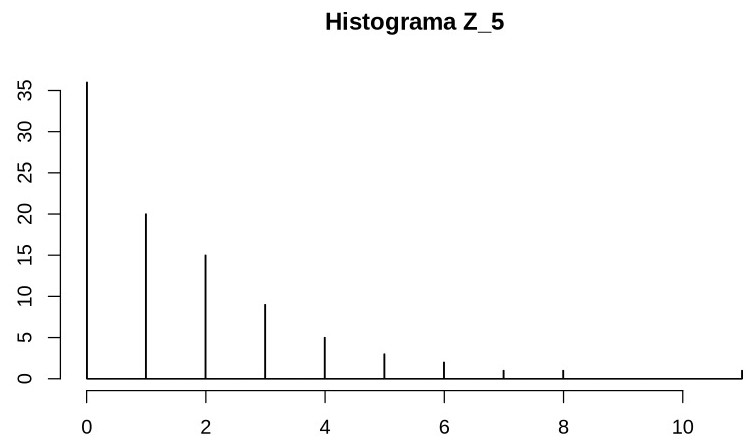
\includegraphics[width=\textwidth]{Imatges/histogramaz5p035.jpg}
    \caption{Histograma de $Z_{5}$}
  \end{subfigure}
  \hfill
  \begin{subfigure}[b]{0.49\textwidth}
    \centering
    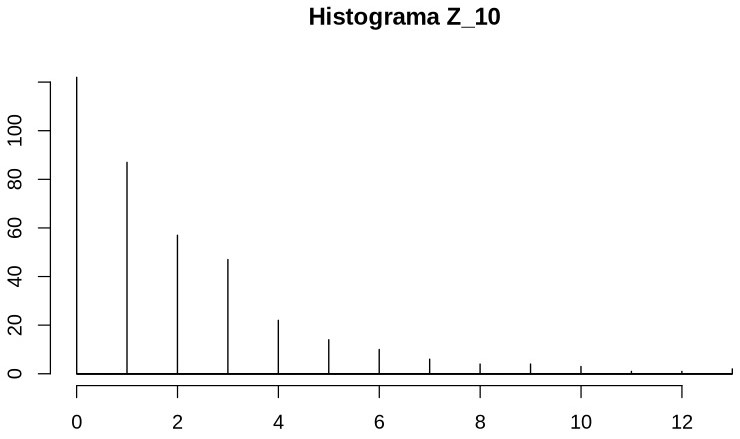
\includegraphics[width=\textwidth]{Imatges/histogramaz10p035.jpg}
    \caption{Histograma de $Z_{10}$}
  \end{subfigure}
  \caption{Histogrames de la cinquena i desena generacions amb probabilitat $p=0,35$.}
\end{figure}
Veiem que com és esperat, en els dos histogrames s'observa que els valors més petits surten amb molta més freqüència que els valors més grans, cal destacar que són dos histogrames de dues generacions de números concretes, però aquest comportament és característic de totes les generacions.\\
Fixant ara $p=\frac{1}{2}$ realitzem un histograma de la desena generació, utilitzant el mateix codi per a la realització dels altres histogrames.
\newpage
\begin{center}
  \begin{lstlisting}[language=R, caption={Histograma de la desena generació amb probabilitat p=0,5},xleftmargin=.0\textwidth,xrightmargin=.0\textwidth]
n=11; c=1:n; c[n-1]=0
while(c[n-1]==0){ for(i in 1:(n-2)){ c[i+1]=sum(rgeom(c[i], 0.5)) } }
mostra=rgeom(c[n-1], 0.5)
hist(mostra, breaks=seq(0,max(mostra),1/length(mostra)), freq=FALSE, xlab="", 
     ylab="", ylim=c(0,max(table(mostra))), main = "Histograma Z_n")
\end{lstlisting}
\end{center}

\begin{center}
  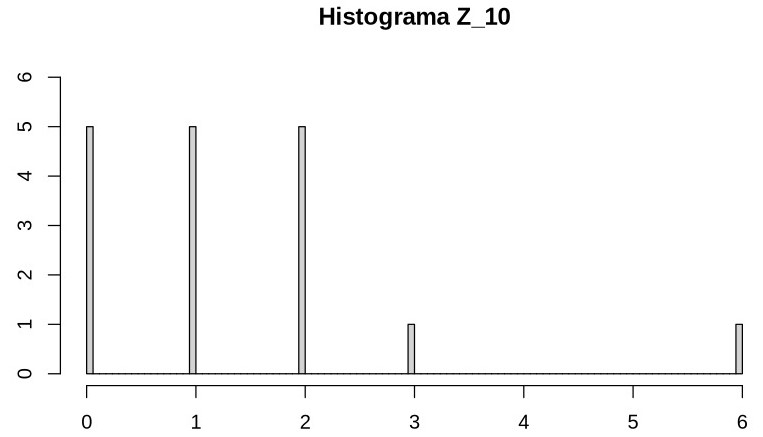
\includegraphics[scale=0.5]{Imatges/histogramaz10p05.jpg}\\
  \figurename{ : Histograma de $Z_{10}$ amb $p=\frac{1}{2}$}
\end{center}

S'observa una repartició més homogènia entre els primers termes que a l'histograma de $Z_{10}$ amb $p=0.35$. Aquest fet és degut a que al augmentar la probabilitat d'èxit $p$ també augmenta la probabilitat $\mathbb{P}(X=k)=(1-p)^{k}p$ per a $k=0,1$, en canvi per a $k>1$ la probabilitat disminueix, és a dir:
$(1-0.35)^{0}0.35=0.35<0.5=(1-0.5)^{0}0.5, (1-0.35)^{1}0.35=0.2275<0.25=(1-0.5)^{1}0.5, (1-0.35)^{2}0.35=0.147875>0.125=(1-0.5)^{2}0.5, (1-0.35)^{3}0.35=0.09611875>0.0625=(1-0.5)^{3}0.5$.

\end{document}
